\documentclass{article}
\usepackage[utf8]{inputenc}
\usepackage{geometry}
\usepackage{graphicx}
\usepackage{amsmath}
\usepackage{amsfonts}
\usepackage{amsthm}
\usepackage{amssymb}
\usepackage[most]{tcolorbox}
\usepackage{array}
\usepackage{latexsym}
\usepackage{alltt}
\usepackage{hyperref}
\usepackage{color, colortbl}
\usepackage{float}
\usepackage{pdfpages}
\usepackage{algpseudocode}
\usepackage{multicol}
\usepackage{multirow}
\usepackage{caption}
\usepackage{xparse}
\usepackage{setspace}
\usepackage{enumitem}
\usepackage{pdflscape}
% \usepackage{parskip}
\usepackage{blindtext}
\usepackage{forest}
\usepackage[newfloat]{minted}
\usepackage{booktabs}


\geometry
{
  a4paper,
  left=12mm,
  right=12mm,
  top=12mm,
  bottom=15mm,
}

% mybox
\newtcolorbox{mybox}[3][]
{
  colframe = #2!25,
  colback  = #2!10,
  coltitle = #2!20!black,  
  title    = {#3},
  #1,
}

\definecolor{ex}{rgb}{1.00,0.65,0.00}
\definecolor{bg}{rgb}{0.95,0.95,0.95}
\setminted
{
	mathescape=true,
	xleftmargin=\parindent,
	bgcolor=bg,
	escapeinside=@@
}

\SetupFloatingEnvironment{listing}{name=Code}

\usetikzlibrary{patterns,positioning,fit,arrows,calc,shapes.geometric,shapes.multipart,decorations.pathreplacing}

% New environments that use mybox
\newcounter{example}[section]
\newenvironment{example}[1]{\begin{mybox}[breakable]{ex}{\refstepcounter{example}\textbf{Example \thesection.\theexample #1}}}{\end{mybox}}

\newcounter{definition}[section]
\newenvironment{definition}[1]{\refstepcounter{definition}\begin{mybox}[breakable]{blue}{\textbf{Definition \thesection.\thedefinition #1}}}{\end{mybox}}

\newcounter{theorem}[section]
\newenvironment{theorem}[1]{\begin{mybox}{red}{\refstepcounter{theorem}\textbf{Theorem \thesection.\thetheorem #1}}}{\end{mybox}}

\newenvironment{formula}[1]{\begin{mybox}{cyan}{\textbf{#1}}}{\end{mybox}}

% Changing maketitle
\makeatletter         
\renewcommand\maketitle{
{\raggedright % Note the extra {
\begin{center}
{\Large \bfseries \@title}\\[2ex] 
{\large \@author \ - \@date}\\[2ex]
\end{center}}} % Note the extra }
\makeatother

% \onehalfspacing % adjust spacing
\setlength{\parskip}{0.5\baselineskip}

% macros
\newcommand{\prob}[1]{\textbf{\textit{P}}\left\{#1\right\}}
\newcommand{\expc}[1]{\mathbf{E}\left(#1\right)}
\newcommand{\expcs}[1]{\mathbf{E}^2\left(#1\right)}
\newcommand{\var}[1]{\text{Var}\left( #1 \right)}
\newcommand{\ra}{\rightarrow}
\newcommand{\Ra}{\Rightarrow}
\newcommand{\R}[2]{\tikz [remember picture,overlay] \node (#1) {#2};}

\def\circtxt#1{$\mathalpha \bigcirc \mkern-13mu \mathtt #1$}
\def\smiley{\textcircled{\scriptsize $\mkern3mu\ddot{\ } \mkern-15mu \smallsmile$}}


\NewDocumentCommand{\dsum}{%
    e{^_}
}{%
  {% 
    \displaystyle\sum
    \IfValueT{#1}{^{#1}}
    \IfValueT{#2}{_{#2}}
  }
}%

% maketitle variables
\title{CENG 242 - Chapter 9: Control Flow}
\author{Burak Metehan Tunçel}
\date{May 2022}

\begin{document}

\maketitle

\begin{figure}[ht]
  \centering
  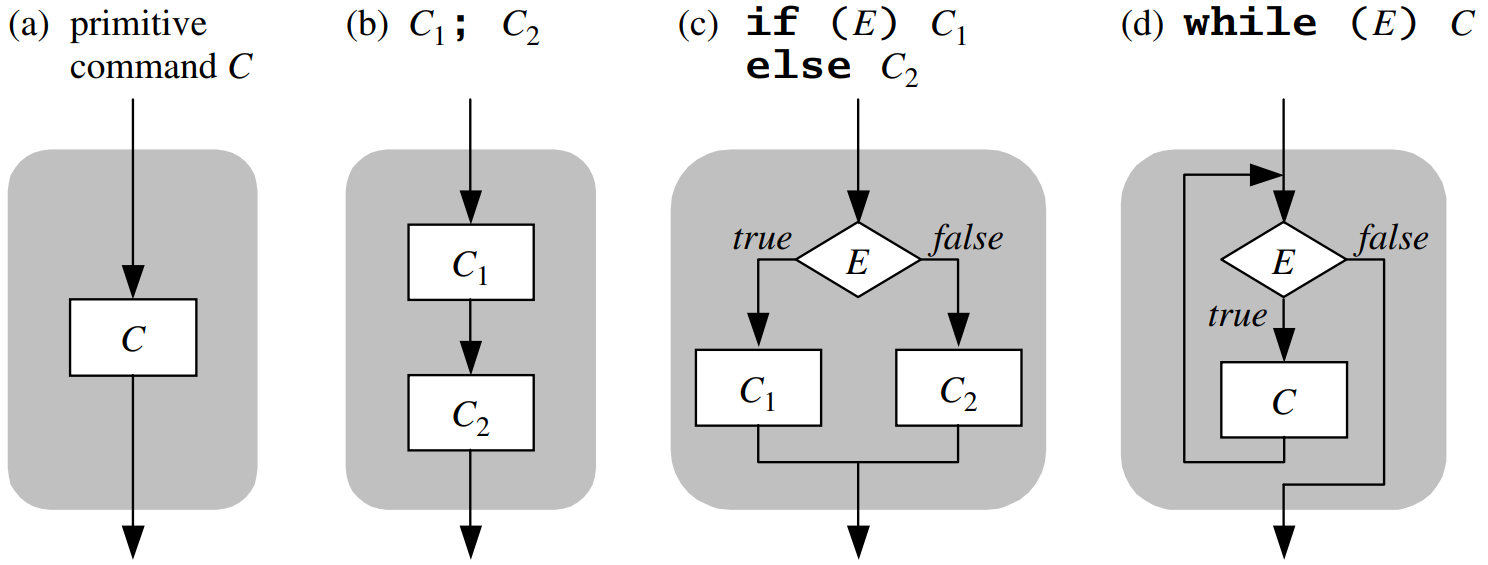
\includegraphics[width=.67\textwidth]{img/fig-9.1.png}
  \caption{Flowcharts of primitive, sequential, if-, and while-commands.}
\end{figure}

\begin{multicols*}{2}
\setlength{\columnsep}{1.5cm}
\setlength{\columnseprule}{0.2pt}

\section{Sequencers}
\label{sec:sequencers}

Figure 1 shows four flowcharts: a \textit{simple command}, a \textit{sequential subcommand}, an \textit{if-command}, and a \textit{while-command}. Each of these flowcharts has a single entry and a single exit. The same is true for other conditional commands, such as case commands, and other iterative commands, such as for-commands. It follows that \textit{any} command formed by composing simple, sequential, conditional, and iterative commands has a single-entry single-exit control flow.

Sometimes we need to implement more general control flows. In particular, single-entry multi-exit control flows are often desirable.

A \textit{\textbf{sequencer}} is a construct that transfers control to some other point in the program, which is called the sequencer's \textit{\textbf{destination}}. Using sequencers we can implement a variety of control flows, with multiple entries and/or multiple exits. We shall examine several kinds of sequencers:
\setlength{\columnsep}{0cm}
\setlength{\columnseprule}{0pt}
\begin{multicols}{3}
  \begin{itemize}[leftmargin=4pt]
    \item jumps
    \item escapes
    \item exceptions 
  \end{itemize}
\end{multicols}
\setlength{\columnsep}{1.5cm}
\setlength{\columnseprule}{0.2pt}
This order of presentation follows the trend in language design from low-level sequencers (jumps) towards higher-level sequencers (escapes and exceptions).

Some kinds of sequencers are able to \textit{\textbf{carry}} values. Such values are computed at the place where the sequencer is executed, and are available for use at the sequencer's destination.


\section{Jumps}
\label{sec:jumps}

A \textit{\textbf{jump}} is a sequencer that transfers control to a specified program point. A jump typically has the form ``\texttt{goto $L$;}'', and this transfers control directly to the program point denoted by $L$, which is a \textit{\textbf{label}}.

\vspace*{\fill}
\columnbreak

\begin{formula}{}
\begin{listing}[H]

\begin{minted}[bgcolor={}]{c}
@\R{l1}{}@L1:  x++;
      if (x>10) goto L2@\R{gl2}{}@;
      j++;
      for (i=0;i<j;j++) {
          x=x*2;
@\R{l2}{}@L2:      if (x>1000) goto L3@\R{gl3}{}@;
          else goto L1@\R{gl1}{}@;
      }
@\R{l3}{}@L3:  printf("out\n");
\end{minted}

\begin{tikzpicture} [thick,remember picture,overlay,rounded corners=3pt]
  \draw [green,->] (gl1) -- +(0,3) -| (l1);
  \draw [violet,->] (gl2) -- +(0,-0.55) -|  (l2);
  \draw [red,->] (gl3) -- +(0,-1.7) -| (l3);
\end{tikzpicture}

\caption{}
\label{code:code1}

\end{listing}
\end{formula}

Unrestricted jumps allow any command to have multiple entries and multiple
exits. They tend to give rise to ``spaghetti'' code, so called because its flowchart is tangled. Also, ``spaghetti'' code tend to be hard to understand and is prone to errors.
\begin{listing}[H]

\begin{minted}{c}
L1: ...
  goto L2;        @\color{violet}\circtxt{1}@
  ...
  for (i=0;i<10;i++) {
    int x=t;
L2: ...
    goto L1;    @\color{violet}\circtxt{2}@
    ...
	  goto L2:    @\color{violet}\circtxt{3}@
  }
\end{minted}

\caption{}
\label{code:code2}
\end{listing}

Also, when we consider the jumps, lifetime and values of local variables and values of index variables become a problem.

In \texttt{C}, labels are local to enclosing block. No jumps allowed into the block or out the block. Newer languages avoid jumps.

Jump is avoided but single entrance multiple exit is still desirable. It can be satisfied by \textbf{escapes}.


\section{Escapes}
\label{sec:escapes}

An \textit{\textbf{escape}} is a sequencer that terminates execution of a textually enclosing command or procedure. In terms of a flowchart, the destination of an escape is always the exit point of an enclosing subchart. With escapes we can program \textit{single-entry multi-exit control flows}.

\noindent Depending on which enclosing block to jump out of:
\begin{itemize}
  \item loop: \textcolor{ex}{break} sequencer.
  \item loops: \textcolor{ex}{exit} sequencer.
  \item function: \textcolor{ex}{return} sequencer.
  \item program: \textcolor{ex}{halt} sequencer.
\end{itemize}

\subsection{Break Sequencer}
\label{subsec:break-seq}

break sequencer in C, C++, Java terminates the innermost
enclosing loop block.

The break sequencer of \texttt{C}, \texttt{C++}, and \texttt{JAVA} allows any composite command (typically a loop or switch command) to be terminated immediately.

\begin{itemize}
  \item \textcolor{ex}{break sequencer} in \texttt{C}, \texttt{C++}, \texttt{Java} terminates the innermost enclosing loop block.
  \item \textcolor{ex}{continue} in \texttt{C}, \texttt{C++} stays in the same block but ends current iteration.
  \item \textcolor{ex}{exit sequencer} in \texttt{Ada} or labeled \texttt{break} in Java can terminate multiple levels of blocks by specifying labels. Java code:
\begin{listing}[H]
\begin{minted}[breaklines]{java}
  L1: for (i = 0; i < 10; i++) {
        for (j = i; j < i; j++) {
          if (...) break;
          else if (...) continue;
          else if (...) break L1;
          else if (...) continue L1;
          s += i*j;
        }
      }
\end{minted}
\caption{}
\label{code:code3}
\end{listing}     

  \item \textcolor{ex}{return sequencer} exist in most languages for terminating the innermost function block.
  \item \textcolor{ex}{halt sequencer} either provided by operating system or PL terminates the program.
\end{itemize}

Consider jump inside of a block or jump out of a block for the function case:
\begin{listing}[H]
\begin{minted}[breaklines]{c}
int f(int n) {
    int a;

L1: if (n<0) goto L2;   @\color{violet}\circtxt{1}@
    else if (n=1) return 1;
    else return f(n-1)*n;
}

int main() {
    ...
    f(12);
L2: ....
    goto L1:             @\color{violet}\circtxt{2}@
    }
\end{minted}
\caption{Jump out of a function block, jump inside of a function block}
\label{code:code4}
\end{listing} 

Jumps update current instruction pointer. But what about environment, activation record (run-time stack)? Jumping outside or inside a function block is possible only for one direction if stack position can be
recovered. Called \textit{non-local jumps}.

% \begin{figure}[T]
%   \centering
%   \begin{tikzpicture}
%     [stack/.style={rectangle split, rectangle split parts=4,draw,
%       text width=7em},
%       scolor/.style={rectangle split part fill={white,blue!20!white,blue!20!white,blue!20!white}}]

%     \node [stack,scolor] (stk1) {
%       \nodepart{one} \rule{0pt}{3em}
%       \nodepart{two} record of f()
%       \nodepart{three} record of g()
%       \nodepart{four} record of main()
%     };

%     \node [stack,scolor,rectangle split parts=3, right=5em of stk1] (stk2) {
%       \nodepart{one} \rule{0pt}{4.7em}
%       \nodepart{two} record of g()
%       \nodepart{three} record of main()
%     };

%     \node [stack,scolor, rectangle split parts=3,right=5em of stk2] (stk3) {
%       \nodepart{one} \rule{0pt}{4.7em}\hspace*{2em} ??
%       \nodepart{two} record of g()
%       \nodepart{three} record of main()
%     };

%     \draw [->,green,thick] (stk1.two east) -- +(1em,0) |- (stk2.two west);
%     \draw [->,red,thick] (stk2.two east) -- +(1em,0) node [fill=white, yshift=.9em] {$\times$} |-  ($(stk3.one west) - (0,1.6em)$);
%   \end{tikzpicture}
%   \caption
% \end{figure}

Non-local jumps can be useful in unexpected error occuring inside of many levels of recursion in order to jump to the outer-most related caller function. Instead of jumping, it can be satisfied by \textbf{exceptions}.


\section{Exceptions}
\label{sec:exceptions}

An \textit{\textbf{abnormal situation}} is one in which a program cannot continue normally. Typical examples are the situations that arise when an arithmetic operation overflows, or an input/output operation cannot be completed.

What should happen when such an abnormal situation arises? Too often, the program simply halts with a diagnostic message. It is much better if the program transfers control to a \textit{handler}, a piece of code that enables the program to recover from the situation. A program that recovers reasonably from such situations is said to be \textit{robust}.

Exceptions are a superior technique for handling abnormal situations. An \textit{\textbf{exception}} is an entity that represents an abnormal situation (or a family of abnormal situations). Any code that detects an abnormal situation can \textit{\textbf{throw}} (or \textit{raise}) an appropriate exception. That exception may subsequently be \textit{\textbf{caught}} in another part of the program, where a construct called an \textit{\textbf{exception handler}} (or \textit{just handler}) recovers from the abnormal situation.

Every exception can be caught and handled, and the programmer has complete control over where and how each exception is handled. Exceptions cannot be ignored: if an exception is thrown, the program will halt unless it catches the exception.

The first major programming language with a general form of exception handling was \texttt{PL/I}. Then, a better exception concept has been designed into more modern languages such as \texttt{C++} and \texttt{JAVA}.

A handler for any exception may be attached to any command. If that command (or any procedure called by it) throws the exception, execution of that command is terminated and control is transferred to the handler. The command that threw the exception is never resumed.

We can attach different handlers for the same exception to different commands in the program. We can also attach handlers for several different exceptions to the same command.

\noindent Note the following important properties of exceptions:
\begin{itemize}
  \item If a subcommand throws an exception, the enclosing command also throws that exception, unless it is an exception-handling command able to catch that particular exception. If a procedure's body throws an exception, the corresponding procedure call also throws that exception.
  \item A command that throws an exception is terminated abruptly (and will never be resumed).
  \item Certain exceptions are built-in, and may be thrown by built-in operations. Examples are arithmetic overflow and out-of-range array indexing.
  \item Further exceptions can be declared by the programmer, and can be thrown explicitly when the program itself detects an abnormal situation.
\end{itemize}
\texttt{C++} and \texttt{JAVA}, being object-oriented languages, treat exceptions as objects. \texttt{JAVA}, for instance, has a built-in \texttt{Exception} class, and every exception is an object of a subclass of \texttt{Exception}. Each subclass of \texttt{Exception} represents a different abnormal situation. An exception object contains an explanatory message (and possibly other values), which will be carried to the handler. Being first-class values, exceptions can be stored and passed as parameters as well as being thrown and caught.

The \texttt{JAVA} sequencer ``\texttt{throw $E$;}'' throws the exception yielded by expression $E$. The \texttt{JAVA} exception-handling command has the form:
\begin{minted}[escapeinside=\#\#]{java}
try { #$C_0$#; }
catch { (#$T_1$# #$I_1$#) #$C_1$#; }
...
catch { (#$T_n$# #$I_n$#) #$C_n$#; } 
finally { #$C_f$#; }
\end{minted}
this is able to catch any exception of class $T_1$ or $\ldots$ or $T_n$. If the subcommand $C_0$ throws an exception of type $T_i$, then the exception handler $C_i$ is executed with the identifier $I_i$ bound to that exception. Just before the exception-handling command terminates (whether normally or abruptly), the subcommand $C_f$ is executed unconditionally. (The \texttt{\textbf{finally}} clause is optional.)

\vspace*{\fill}
\columnbreak

\subsection{From Lecture Slides}
\label{subsec:from-lecture-slides}

\subsubsection{Exception}
\label{subsubsec:slide-exception}

Exceptions are controlled jumps out of multiple levels of function calls to an outer control point (\texttt{handler} or \texttt{catch}). \texttt{C} does not have exceptions but non-local jumps possible via \texttt{setjmp()}, \texttt{longjmp()} library calls. However, \texttt{C++} and \texttt{Java} has ``\texttt{try $\{$...$\}$ catch(...) $\{$...$\}$}''.

Each \texttt{try-catch} block introduces a non-local jump point. \texttt{try} block is executed and whenever a \texttt{throw {\em expr\/}} command is called in any functions called (even indirectly) inside \texttt{try}  block execution jumps to the \texttt{catch()} part. \texttt{try-catch} blocks can be nested. Execution jumps to closes \texttt{catch} block with a matching type in the parameters with the thrown expression.

\noindent Conventional error handling. Propagate errors with return values.
\begin{listing}[H]

\begin{minted}{c}
int searchopen(char *f) { ...
  /* if search fails $\textnormal{\textcolor{red}{error occurs here}}$ */
  return -5; @\R{e1}{}@ ...
  }
int openparse(char *f) { ...
  if ((r = searchopen(f))<0) @\R{e2}{}@
    return r;@\R{e3}{}@
  else ...
}
int main() {  ...
  if ((rv=openparse("file.txt"))<0) @\R{e4}{}@
    /* $\textnormal{\textcolor{red}{handle error here}}$ */
}
\end{minted}

\begin{tikzpicture} [remember picture, overlay, thick]
  \draw [->,blue] (e1) -- +(4,0) |- (e2);
  \draw [->,blue] (e3) -- +(5,0) |- (e4);
\end{tikzpicture}

\caption{}
\label{code:code5}
\end{listing}

\noindent Error handling with \texttt{try-catch}. (based on run-time stack)
\begin{listing}[H]
\begin{minted}{cpp}
enum Exception { NOTFOUND, ..., PERMS};
void searchopen(char *f) { ...
  /* if open fails $\textnormal{\textcolor{red}{error occurs here}}$ */
  throw PERMS; @\R{ee1}{}@ ...
}
void openparse(char *f) { ...
  searchopen(f); ...
}
int main() {  ...
  try {...
    openparse("file.txt"); ...
  } catch(Exception e) {@\R{ee4}{}@
    /* $\textnormal{\textcolor{red}{handle error here}}$ */
  } ...
}
\end{minted}

\tikz [remember picture, overlay,blue] \draw [->,thick] (ee1) -- +(4,0) |- (ee4);

\caption{}
\label{code:code6}
\end{listing}

\end{multicols*}

\noindent Nested exceptions are handled based on types. \texttt{C++}:
\begin{listing}[ht]

\begin{minted}{cpp}
int main() {... 
  try { C1;  f@\R{tf}{}@() ; C2 } 
  catch (double@\R{cdoub}{}@ a) {...}
}

void f@\R{ff}{}@() {...; 
  try {...; g@\R{tg}{}@() ; ... } catch (int@\R{cint}{}@ a) {...} 
}

void g@\R{fg}{}@() {...; 
  throw 4@\R{tint}{}@; ... ; throw 1.5@\R{tdoub}{}@; ...
}
\end{minted}

\begin{tikzpicture} [remember picture,overlay, thick] 
  \draw [->,blue] (tf) -- +(0,-1) -| node [fill=blue!5!white,pos=0.2] {\tiny call}  (ff);
  \draw [->,blue] (tg) -- +(0,-0.4) -| node [fill=blue!5!white,pos=0.2] {\tiny call} (fg);
  \draw [->,red] (tint) -- +(0,1) -|  node [fill=blue!5!white,pos=0.2] {\tiny exception} (cint);
  \draw [->,red] (tdoub) -- +(0,2.5) -| node [fill=blue!5!white,pos=0.2] {\tiny exception} (cdoub);
\end{tikzpicture}

\caption{}
\label{code:code7}
\end{listing}

\noindent In case no handlers found a run time error generated. Program halts.

\subsubsection{Co-routines}
\label{subsubsec:slide-coroutine}

\begin{itemize}
  \item \textit{\textbf{Sequential flow:}} local jumps, subroutine calls, exceptions
  \item \textit{\textbf{Concurrent flow:}} multiple contexes (stack and instruction pointer). Execution switches between them.
  \item \textit{\textbf{Multiple uses:}} \textcolor{red}{callbacks}, \textcolor{red}{generators} (iterators), \textcolor{red}{threads}, \textcolor{red}{fibers}, \textcolor{red}{asynchronous}, \textcolor{red}{event based}, or \textcolor{red}{concurrent} programming
  \item Non-local jumps to different environments guided coordinated programs or a global scheduling mechanism:

  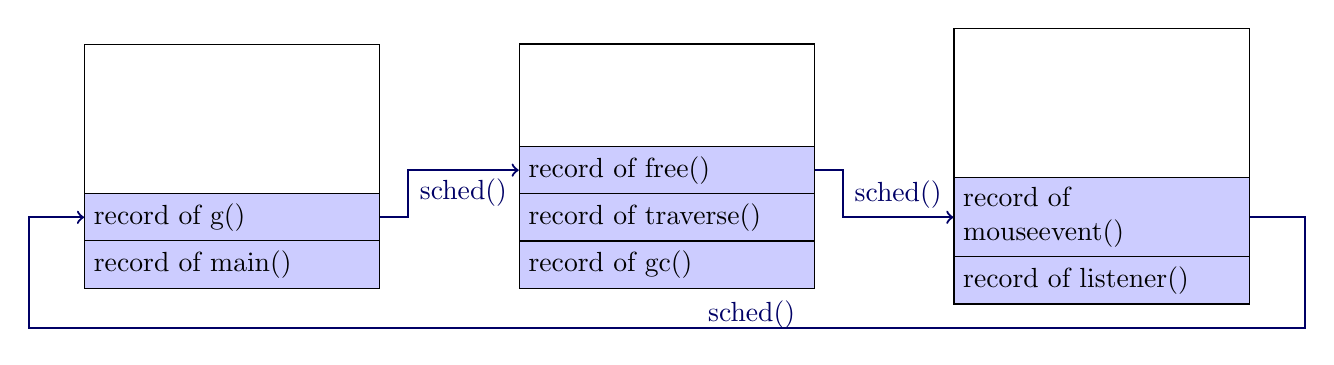
\begin{tikzpicture}
    [stack/.style={rectangle split, rectangle split parts=4,draw,
      text width=10em},
      scolor/.style={rectangle split part fill={white,blue!20!white,blue!20!white,blue!20!white}}]
  
    \node [stack,scolor,rectangle split parts=3] (stk2) {
      \nodepart{one} \rule{0pt}{4.7em}
      \nodepart{two} record of g()
      \nodepart{three} record of main()
    };
  
    \node [stack,scolor,right=5em of stk2] (stk1) {
      \nodepart{one} \rule{0pt}{3em}
      \nodepart{two} record of free()
      \nodepart{three} record of traverse()
      \nodepart{four} record of gc()
    };
  
    \node [stack,scolor, rectangle split parts=3,right=5em of stk1] (stk3) {
      \nodepart{one} \rule{0pt}{4.7em}\hspace*{2em}
      \nodepart{two} record of mouseevent()
      \nodepart{three} record of listener()
    };
  
    \draw [->,blue!40!black,thick] (stk2.two east) -- +(1em,0) node [xshift=2em, yshift=.9em] {sched()} |- (stk1.two west);
  
    \draw [->,blue!40!black,thick] (stk1.two east) -- +(1em,0) node [xshift=2em, yshift=-.9em] {sched()} |-  (stk3.two west);
  
    \draw [->,blue!40!black,thick] (stk3.two east) -- +(2em,0) -- +(2em,-4em)  node [xshift=-20em, yshift=.5em] {sched()} -| ($(stk2.two west)+(-2em,0)$) --  (stk2.two west);
  \end{tikzpicture}
\end{itemize}


% \end{multicols*}

\end{document}
